\section{{\prg mcdiff}\index{mcdiff} - calculate and fit  magnetic Neutron or Resonant Xray 
Scattering}\label{mcdiff}

In order to calculate neutron diffraction and resonant magnetic Xray scattering
at a specified temperature and magnetic field you can use the module {\prg mcdiff\index{mcdiff}}.
An input file {\prg mcdiff.in } for this program can be easily created from
the output file {\prg mcphas.sps} by the program {\prg setup\_mcdiff\_in\index{setup\_mcdiff\_in}}
(in {\prg mcdiff.in } structural data of non magnetic atoms and wavelength
                        and maximal angle have to be edited).
\footnote{Alternatively, one may make use of the program {\prg spins\index{spins}}.} 
{\prg mcdiff\index{mcdiff}} then calculates neutron reflection and intensity list.
Miller indices always refer to the lattice $\vec a^*, \vec b^*, \vec c^*$, which
is the reciprocal lattice of $\vec a, \vec b, \vec c$ as defined by lattice
parameters $a,b,c$ and angles $\alpha,\beta,\gamma$.

Here follows an example input file (see examples/ndcu2b\_new/mcdiff\index{mcdiff}.in):

{\footnotesize
\begin{verbatim}
#
#<!--mcdiff.mcdiff.in>
#***************************************************************
#      mcdiff is a program for the calculation of elastic
#   neutron diffraction and resonant magnetic Xray scattering 
#  reference: M. Rotter and A. Boothroyd PRB 79 (2009) 140405R
#*************************************************************** 
# this input file contains 4 sections corresponding to different
# groups of parameters
#
# - all lines have to start with a # sign with the  exception of 
#   the lines containing atomic positional parameters
# - the other parameters have to be defined in the corresponding 
#   section by statements such as parameter=value
# - the sequence of the parameters within a section is arbitrary
# 
#
# %SECTION 1%  OVERALL PARAMETERS
#
#! lambda   = 2.3587  wavelength (A)
#
#! thetamax = 10   maximum bragg angle (deg)
#
#! ovalltemp= 0  overall temperature factor (A^2) 
#           ...I ~ EXP(-2 * ovalltemp * sintheta^2 / lambda^2) 
#                  relation to other notations:
#                  ovalltemp = Biso = 8 pi^2 Uiso^2
#
#! lorentz=0  type of lorentzfactor to be used
#            0.....no lorentzfactor 
#            1.....neutron powder flat sample
#            2.....neutron powder cylindrical sample
#            3.....neutron single crystal
#            4.....neutron TOF powder cyl. sample - d-pattern log scaled
#            5.....neutron TOF powder cyl. sample - d-pattern normal scaled
#
#     out* controls the type of output in user defined column * of mcdiff.out
#! out4=30    (optional)
#! out5=31    (optional)
#! out6=32    (optional)
#! out10=1    (optional)
#! out11=0    (optional)
#     ... in out*=n the numbers n have the following meaning:
#            0....LF          
#            1....|NSF|[b]    
#            2....Re(NSF)[b]  
#            3....Im(NSF)[b]  
#            4....|MSF|       
#            5....|MSF.P|     
#            6....Re(MSF.P)   
#            7....Im(MSF.P)   
#            8....|MSFdip|    
#            9....|MSFdip.P|  
#            10....Re(MSFdip.P)
#            11....Im(MSFdip.P)
#            12....angl(Q,P)[�]
#            13....i(MSFxMSF*).P
#            14....I+          
#            15....I-          
#            16....I+/I-       
#            17....i(MSFxMSF*)dip.P
#            18....Idip+       
#            19....Idip-       
#            20....Idip+/Idip- 
#            21....2*|MSF.P|/sin^2(angl(Q,P)
#            22....2*|MSFdip.P|/sin^2(angl(Q,P)
#            23....2|NSF|sqrt(4PI/3.65)(|g|-sqrt(g^2-1/sin(angl(Q,P))))_with_g=(1+I+/I-)/(1-I+/I-)
#            24....2|NSF|sqrt(4PI/3.65)(|g|+sqrt(g^2-1/sin(angl(Q,P))))_with_g=(1+I+/I-)/(1-I+/I-)
#            25....2|NSF|sqrt(4PI/3.65)(|g|-sqrt(g^2-1/sin(angl(Q,P))))_with_g=(1+Idip+/Idip-)/(1-Idip+/Idip-)
#            26....2|NSF|sqrt(4PI/3.65)(|g|+sqrt(g^2-1/sin(angl(Q,P))))_with_g=(1+Idip+/Idip-)/(1-Idip+/Idip-)
#            27....Qx[1/A]     
#            28....Qy[1/A]     
#            29....Qz[1/A]     
#            30....d[A]        
#            31....|Q|[1/A]    
#            32....2theta      
#
#           In the above the intensities I+ and I- are the spinflip and nonspinflip intensities
#           in a polarised neutron experiment:
#            I+-=LF exp(-OTF Q^2/8pi^2) 
#                    [ |NSF/NB|^2 + 3.65/4pi (|MSF|^2-+i(MSF x MSF*).P)/NB^2 
#                        +-  sqrt(3.65/4pi)/NB^2 (NSF (MSF*.P) + NSF* (MSF.P)]
#           LF  ..... Lorentzfactor
#           MSF ..... magnetic structure factor
#           NSF ..... nuclear structure factor
#
#
#             For some of the above options we need the
#! Pa=  0.0000   Components of Polarisation Vector in terms of lattice vectors P=(Pa * a + Pb * b + Pc *c)
#! Pb=  0.0000   Note: the length of P, i.e. |P| indicates the degree of beam polarisation (|P|<=1)
#! Pc=  1.0000
#
#
# %SECTION 2% LIST OF NONMAGNETIC ATOMS IN CRYSTALLOGRAPHIC UNIT CELL
#
#
#! natcryst=0      number of nonmagnetic atoms in primitive crystalographic unit cell
#
# it follows a list of natcryst lines with nonmagnetic atoms
# ... notes: - if an occupancy other than 1.0 is needed, just reduce 
#              the scattering length linear accordingly
#            - Debye Waller Factor notation: sqr(Intensity) ~ structure factor ~ 
#              ~sum_n ()n exp(-2 DWFn sin^2(theta) / lambda^2)=EXP (-Wn),  
#              relation to other notations: 2*DWF = B = 8 pi^2 <u^2>, units DWF (A^2)
#
#! use_dadbdc=0
#            - 0 means: da db and dc are not used by the program (unless you enter a line #! use_dadbdc=1),
#               dr1,dr2 and dr3 refer to the primitive lattice given below
# Real Imag[scattering length(10^-12cm)]   da(a)    db(b)    dc(c)    dr1(r1)  dr2(r2)  dr3(r3)  DWF(A^2)
#
#
# %SECTION 3% DESCRIPTION OF THE LATTICE
#
#
# Note: what follows here may directly be taken from the output of program spins 
#       (file spins.out) or charges (file charges.out)
# -----------------------------------------------------------------------------
#
# lattice constants (A) and angles 
#! a=4.3843 b=7.0326 c=7.4194 alpha=  90 beta=  90 gamma=  90
#
# primitive lattice vectors 
#! r1a= 0.500000 r2a= 0.000000 r3a= 0.000000
#! r1b= 0.500000 r2b= 1.000000 r3b= 0.000000   primitive lattice vectors (a)(b)(c)
#! r1c= 0.500000 r2c= 0.000000 r3c= 1.000000
#
#
#
# %SECTION 4% DESCRIPTION OF MAGNETIC UNIT CELL AND LIST OF MAGNETIC ATOMS
#
#
# here follows the description of the magnetic unit cell with respect
# to the primitive crystallographic unit cell:
# 'nr1', 'nr2', 'nr3' ...the crystallographic unit cell has to be taken 
#                        nr1 nr2 and nr3 times along r1 r2 and r3,
#                        respectively to get magnetic unit cell
# 'nat' denotes the number of magnetic atoms in magnetic unit cell
#
# Temperature,  External Magnetic Field: Magnetic Unit Cell
#! T=1.5 K Ha=0 T Hb= 0 T Hc= 0 T: nr1=10 nr2=1 nr3=1 nat=20 
#
#
# It follows a list of nat lines with to describe the magnetic moment configuration
# Notes:
# 'atom-filename' means the single ion property filename of this magnetic atom:
#                 -it must contain the Formfactor Coefficients (e.g. see international tables)
#                                      Lande factor
#                                      Neutron Scattering Length (10^-12 cm) 
#                 -it may contain a    Debey Waller Factor
# 'da' 'db' and 'dc' are not used by the program (unless you enter a line #! use_dadbdc=1)
# 'dr1','dr2' and 'dr3' refer to the primitive lattice given below
# 'Ma','Mb','Mc' denote the magnetic moment components in Bohr magnetons
#                in case of non orthogonal lattices instead of Ma Mb Mc the components Mx My Mz
#                have to be given, which refer to an right handed orthogonal coordinate system 
#                defined by y||b, z||(a x b) and x normal to y and z
#  <Sa>  <La> <Sb> <Lb >  <Sc> <Lc>  (optional) denote the spin and orbital angular momentum components 
# 'Hxc1' 'Hxc2' 'Hxc3' (optional line, used to go beyond dipole approx for formfactor)
#                                     denote the corresponding exchange fields in meV
#
#{atom-file} da[a]  db[b]    dc[c]     dr1[r1]  dr2[r2]  dr3[r3]   <Ma>     <Mb>     <Mc> [mb] [optional <Sa> <La> <Sb> <Lb> <Sc> <Lc> ]
#{corresponding exchange fields Hxc [meV]- if passed to mcdiff only these are used for calculation (not the magnetic moments)}
{Nd3p.sipf}  0.00000  0.00000  0.00000   0.00000  0.00000  0.00000   +0.00000 +2.09990 +0.00000  +0.00000 +0.00000 -0.78750 +3.67490 +0.00000 +0.00000
{Nd3p.sipf}  0.00000  0.50000  0.07660  -0.00000  0.50000  0.07660   +0.00000 +2.09990 +0.00000  +0.00000 +0.00000 -0.78750 +3.67490 +0.00000 +0.00000
{Nd3p.sipf}  0.50000  0.50000  0.50000   1.00000  0.00000  0.00000   +0.00000 +2.14380 +0.00000  +0.00000 +0.00000 -0.80390 +3.75160 +0.00000 +0.00000
{Nd3p.sipf}  0.50000  1.00000  0.57660   1.00000  0.50000  0.07660   +0.00000 +2.14380 +0.00000  +0.00000 +0.00000 -0.80390 +3.75160 +0.00000 +0.00000
{Nd3p.sipf}  1.00000  1.00000  1.00000   2.00000  0.00000  0.00000   +0.00000 -2.14380 +0.00000  +0.00000 +0.00000 +0.80390 -3.75160 +0.00000 +0.00000
{Nd3p.sipf}  1.00000  1.50000  1.07660   2.00000  0.50000  0.07660   +0.00000 -2.14380 +0.00000  +0.00000 +0.00000 +0.80390 -3.75160 +0.00000 +0.00000
{Nd3p.sipf}  1.50000  1.50000  1.50000   3.00000 -0.00000 -0.00000   +0.00000 -2.09990 +0.00000  +0.00000 +0.00000 +0.78750 -3.67490 +0.00000 +0.00000
{Nd3p.sipf}  1.50000  2.00000  1.57660   3.00000  0.50000  0.07660   +0.00000 -2.09990 +0.00000  +0.00000 +0.00000 +0.78750 -3.67490 +0.00000 +0.00000
{Nd3p.sipf}  2.00000  2.00000  2.00000   4.00000  0.00000  0.00000   +0.00000 +2.11700 +0.00000  +0.00000 +0.00000 -0.79390 +3.70470 +0.00000 +0.00000
{Nd3p.sipf}  2.00000  2.50000  2.07660   4.00000  0.50000  0.07660   +0.00000 +2.11700 +0.00000  +0.00000 +0.00000 -0.79390 +3.70470 +0.00000 +0.00000
{Nd3p.sipf}  2.50000  2.50000  2.50000   5.00000  0.00000 -0.00000   +0.00000 -2.09990 +0.00000  +0.00000 +0.00000 +0.78750 -3.67490 +0.00000 +0.00000
{Nd3p.sipf}  2.50000  3.00000  2.57660   5.00000  0.50000  0.07660   +0.00000 -2.09990 +0.00000  +0.00000 +0.00000 +0.78750 -3.67490 +0.00000 +0.00000
{Nd3p.sipf}  3.00000  3.00000  3.00000   6.00000 -0.00000 -0.00000   +0.00000 -2.14380 +0.00000  +0.00000 +0.00000 +0.80390 -3.75160 +0.00000 +0.00000
{Nd3p.sipf}  3.00000  3.50000  3.07660   6.00000  0.50000  0.07660   +0.00000 -2.14380 +0.00000  +0.00000 +0.00000 +0.80390 -3.75160 +0.00000 +0.00000
{Nd3p.sipf}  3.50000  3.50000  3.50000   7.00000  0.00000  0.00000   +0.00000 +2.14380 +0.00000  +0.00000 +0.00000 -0.80390 +3.75160 +0.00000 +0.00000
{Nd3p.sipf}  3.50000  4.00000  3.57660   7.00000  0.50000  0.07660   +0.00000 +2.14380 +0.00000  +0.00000 +0.00000 -0.80390 +3.75160 +0.00000 +0.00000
{Nd3p.sipf}  4.00000  4.00000  4.00000   8.00000  0.00000  0.00000   +0.00000 +2.09990 +0.00000  +0.00000 +0.00000 -0.78750 +3.67490 +0.00000 +0.00000
{Nd3p.sipf}  4.00000  4.50000  4.07660   8.00000  0.50000  0.07660   +0.00000 +2.09990 +0.00000  +0.00000 +0.00000 -0.78750 +3.67490 +0.00000 +0.00000
{Nd3p.sipf}  4.50000  4.50000  4.50000   9.00000  0.00000  0.00000   +0.00000 -2.11700 +0.00000  +0.00000 +0.00000 +0.79390 -3.70470 +0.00000 +0.00000
{Nd3p.sipf}  4.50000  5.00000  4.57660   9.00000  0.50000  0.07660   +0.00000 -2.11700 +0.00000  +0.00000 +0.00000 +0.79390 -3.70470 +0.00000 +0.00000
\end{verbatim}
}

After issuing the command {\prg mcdiff\index{mcdiff}} 
the program calculates the following output file {\prg results/mcdiff\index{mcdiff}.out}:

{\footnotesize
\begin{verbatim}
#{output file of program mcdiff ./results/mcdiff.out input file: mcdiff.in mcdiff version 3.0 Tue Jun 23 %%@
12:51:43 2009
#!<--mcdiff.mcdiff.out-->
#***********************************************************************
#*
#* mcdiff - program to calculate neutron and magnetic xray diffraction
#*
#* reference: M. Rotter and A. Boothroyd PRB 79 (2009) 140405R
#***********************************************************************
#! unit cell: a= 4.3843 A  b= 4.3843 A c= 2.4194 A  alpha=90  beta=90 gamma=90
#                   /  4.384 A \     /  0.000 A \     /  0.000 A \ 
#                b1=|  0.000 A |  b2=|  4.384 A |  b3=| -0.000 A |
#                   \ -0.000 A /     \  0.000 A /     \  4.839 A /
#! Wavelength=0.9 A   number of atoms: 4
#! T= 2 K Ha= 0 T Hb= 0 T Hc= 0 T
#! Overall temperature factor B=0.3 A^2: Intensity is proportional to exp(-2*B*(sin(theta)/lambda)^2)
# Lorentz Factor: 1 / sin^2(2theta)   neutron powder flat sample
#
# Lorentz Factor not considered for resonant magnetic xray scattering - F1 and F2 transition intensities %%@
calculated
# according to fRMXS as given in equation (2) of Longfield et al. PRB 66 054417 (2002) and maximized with %%@
respect to azimuth.
#
#! nofatoms=4 atoms in unit cell: List of atomic positions dr1 dr2 dr3, moments m scattering lengths sl,
# Debye Waller factor (sqr(Intensity)~|NSF| ~sum_i ()i exp(-2 DWFi sin^2(theta) / lambda^2)=EXP (-Wi),
# units DWF [A^2], relation to other notations 2*DWF=B=8 pi^2 <u^2>)
#  and  Lande factors total angular momentum J (=0 if dipole approximation is used) <j0> and <j2> formfactor
# coefficients
#  dr1[r1]dr2[r2]dr3[r3]ma[MuB]mb[MuB]mc[MuB]sl[10^-12cm]  DWF[A^2] gJ     <j0>:A a      B      b      C      %%@
c      D      <j2>A  a      B      b      C      c      D
#  0.000  0.000  0.000  0.000  0.000 -2.130  0.484+0.000i  0.000  0.857 F(Q)=j0-(1-2/gJ)j2 formfactor for %%@
rare earth/transition metals with gJ=2 0.295 17.685  0.292  6.733  0.431  5.383 -0.019  0.981 18.063  1.841  %%@
7.769  0.991  2.845  0.012 
#  0.000  0.000  0.500  0.000  0.000  2.130  0.484+0.000i  0.000  0.857 F(Q)=j0-(1-2/gJ)j2 formfactor for %%@
rare earth/transition metals with gJ=2 0.295 17.685  0.292  6.733  0.431  5.383 -0.019  0.981 18.063  1.841  %%@
7.769  0.991  2.845  0.012 
#  0.500  0.500  0.250  0.000  0.000  0.000  0.772+0.000i  0.000  0.000  1.000  0.000  0.000  0.000  0.000  %%@
0.000  0.000  0.000  0.000  0.000  0.000  0.000  0.000  0.000 
#  0.500  0.500  0.750  0.000  0.000  0.000  0.772+0.000i  0.000  0.000  1.000  0.000  0.000  0.000  0.000  %%@
0.000  0.000  0.000  0.000  0.000  0.000  0.000  0.000  0.000 
#}
#{h     k      l      d[A]    |Q|[1/A] 2theta  Inuc(2t) Imag(2t) Itot(2t) |NSF|     LF   Imag_dip(2t) %%@
F1:max-Isigpi azim Ipisig azim Ipipig azim F2:max-Isigpi azim Ipisig azim Ipipig azim  |^ma_q| |^mb_q| %%@
|^mc_q| |^ma^2_q||^mb^2_q||^mc^2_q||(^ma*^mb)_q||(^ma*^mc)_q||(^mb*^mc)_q|}
 0.000  0.000  0.500  4.8388  1.2985  10.672   0.0000   0.0000   0.0000   0.0000  29.1583   0.0000        %%@
0.010111 270 0.010111  90 0.000000   0   0.000000 360 0.000000 180 0.000000  90    0.0000   0.0000   1.0652   %%@
0.0000   0.0000   0.0000   0.0000   0.0000   0.0000
 0.000  0.000 -0.500  4.8388  1.2985  10.672   0.0000   0.0000   0.0000   0.0000  29.1583   0.0000        %%@
0.010111  90 0.010111 270 0.000000 360   0.000000 180 0.000000 360 0.000000  90    0.0000   0.0000   1.0652   %%@
0.0000   0.0000   0.0000   0.0000   0.0000   0.0000
 1.000  0.000  0.000  4.3843  1.4331  11.782   0.4935   0.0000   0.4935   0.5760  23.9836   0.0000        %%@
0.000000   0 0.000000   0 0.000000   0   0.013544 314 0.013544 314 0.000571 270    0.0000   0.0000   0.0000   %%@
0.0000   0.0000   2.2691   0.0000   0.0000   0.0000
-1.000  0.000 -0.000  4.3843  1.4331  11.782   0.4935   0.0000   0.4935   0.5760  23.9836   0.0000        %%@
0.000000   0 0.000000   0 0.000000   0   0.013544 314 0.013544 314 0.000571 270    0.0000   0.0000   0.0000   %%@
0.0000   0.0000   2.2691   0.0000   0.0000   0.0000
 0.000  1.000 -0.000  4.3843  1.4331  11.782   0.4935   0.0000   0.4935   0.5760  23.9836   0.0000        %%@
0.000000   0 0.000000   0 0.000000   0   0.013544 314 0.013544 314 0.000571 270    0.0000   0.0000   0.0000   %%@
0.0000   0.0000   2.2691   0.0000   0.0000   0.0000
-0.000 -1.000  0.000  4.3843  1.4331  11.782   0.4935   0.0000   0.4935   0.5760  23.9836   0.0000        %%@
0.000000   0 0.000000   0 0.000000   0   0.013544 314 0.013544 314 0.000571 270    0.0000   0.0000   0.0000   %%@
0.0000   0.0000   2.2691   0.0000   0.0000   0.0000
 1.000  0.000  0.500  3.2490  1.9339  15.923   0.0000   0.4821   0.4821   0.0000  13.2870   0.4821        %%@
0.775763   0 0.775763 180 0.046891  90   0.000000  98 0.000000 278 0.000000   0    0.0000   0.0000   1.0652   %%@
0.0000   0.0000   0.0000   0.0000   0.0000   0.0000
 1.000  0.000 -0.500  3.2490  1.9339  15.923   0.0000   0.4821   0.4821   0.0000  13.2870   0.4821        %%@
0.775763 360 0.775763 180 0.046891 270   0.000000 262 0.000000  82 0.000000 360    0.0000   0.0000   1.0652   %%@
0.0000   0.0000   0.0000   0.0000   0.0000   0.0000
etc ....
-----------------------------------------------------------------------
\end{verbatim}
}

This reflection list contains the Miller indices, the d-spacing, the scattering vector,
the scattering angle 2$\Theta$, nuclear and magnetic neutron scattering intensities
and the corresponding structure-, Lorentzfactor. Moreover it contains the
intensities for the different scattering channels of resonant magnetic x-ray scattering,
the intensity is shown together with the azimuth value where it is maximum. In addition,
the absolute value of the Fourier transform of the magnetic moment components in the different
crystal directions and of some products of the moment components is given.

\subsection{How to generate and view a powder diffraction profile}


.. such a reflection list can be easily transformed into a diffraction pattern
by convolution with the resolution function of a neutron diffractometer.

\begin{itemize}
\item
Simple resolution functions can be easily generated with the help of the programs
{\prg gauss\index{gauss}} and {\prg lorentz\index{lorentz}}. Any other numerical
resolution function, e.g. from a measurement or simulation can be used.
\item
Use program  {\prg convolute\index{convolute}} for doing the convolution. 
Here is an example command: 
{\prg convolute\index{convolute} 6 8  results/mcdiff\index{mcdiff}.out
1 2 resultshb/resolution.dat}
... this gives magnetic pattern such as shown in fig.~\ref{elnpattern}
\item Usually the convolution needs to be done to compare to experimental
data and needs only to be evaluated at the experimental data points, for
example the measured scattering angle values $2\Theta$. This can be 
done by adding a data file to the command,
{\prg convolute\index{convolute} 6 8  results/mcdiff\index{mcdiff}.out
1 2 resultshb/resolution.dat 1 2 datafile.dat}. In our example the
data file contains the experimental data in columns 1 (angle) and columns 2 (Intensity).
\item If needed the resolution function can be stretched using stretching
values given in a separate column of the data file - the command is then
{\prg convolute\index{convolute} 6 8  results/mcdiff\index{mcdiff}.out
1 2 resultshb/resolution.dat 1 2 datafile.dat 13} (in this example the stretching
factor is taken from column 13 of the datafile.
\item Generating of the stretching factor: the stretching factor
may be generated by program {\prg uvw2fwhm\index{uvw2fwhm}} from
the scattering angle values and the parameters U,V and W (as in {\prg FullProf\index{FullProf}}.

\end{itemize}

\begin{figure}[ht]
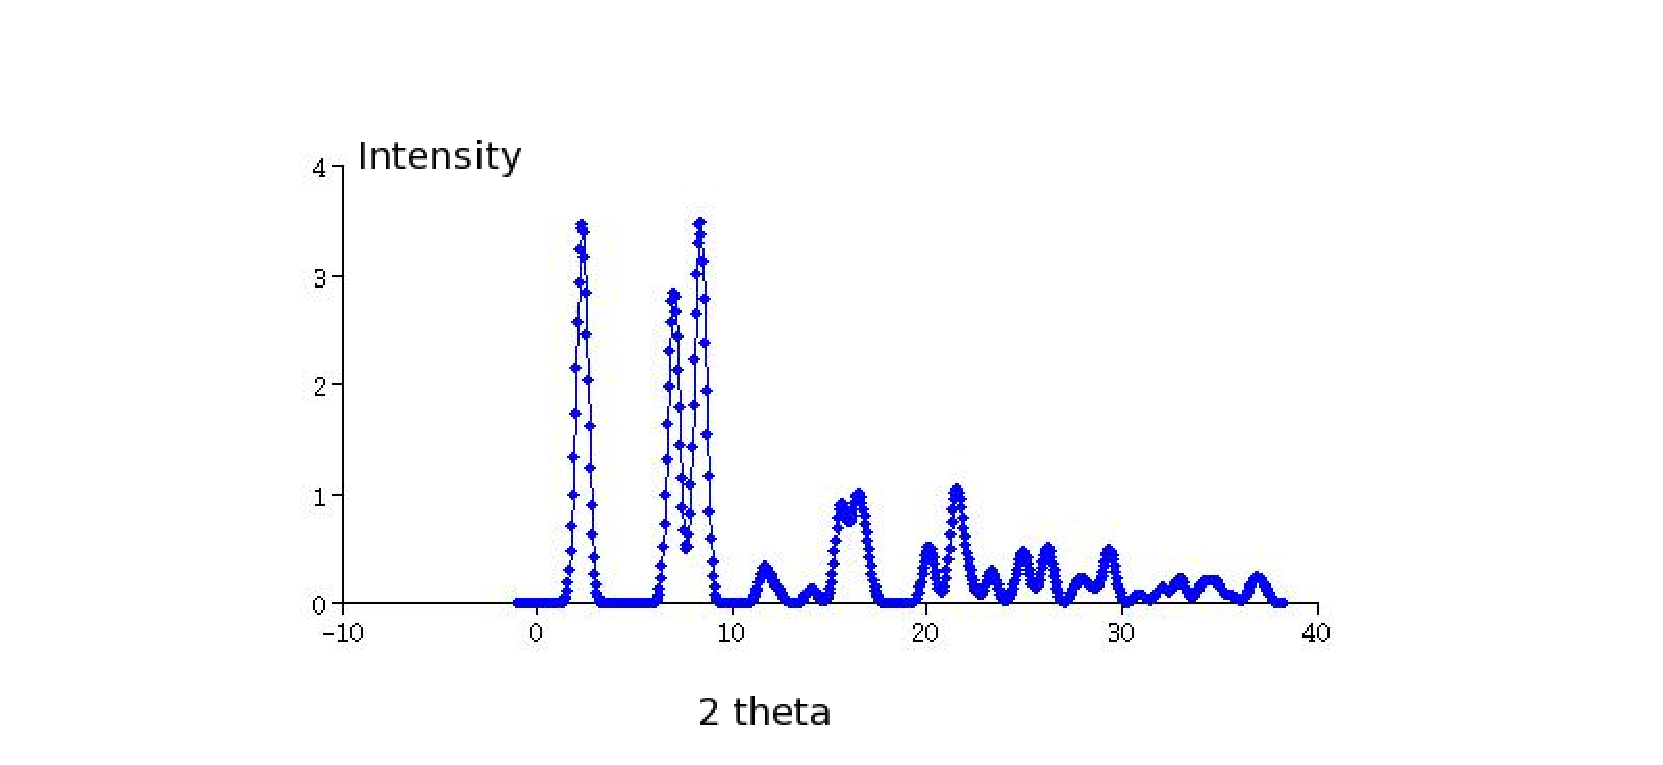
\includegraphics[angle=0,width=1.1\textwidth]{figsrc/patternAF1.eps}
\caption{\label{elnpattern}
Calculated magnetic neutron powder diffraction pattern
of NdCu$_2$~\cite{gratz91-9297} at T=2~K.
[plot created by program {\prg mcdiff\index{mcdiff}+convolute\index{convolute}+display}]}
\end{figure}

\subsection{How to calculate only specific reflections, azimuth dependence and fitting of neutron %%@
intensities}

For the fit of experimental intensities it is often desirable to save computation
time by calculating the intensity only for a specified set of reflections and 
compare it to experimental data. Such list should have the following format

\begin{verbatim}
#{h     k     l }
0.500 0.500 0.500 
0.500 0.500 1.500 
0.500 0.500 2.500 
\end{verbatim}

Lets assume such a list is stored  as file {\prg hkllist.dat}.
Then {\prg mcdiff\index{mcdiff}} can be started as: {\prg mcdiff\index{mcdiff} hkllist.dat}.
The output file will then contain the azimuth dependence of the magnetic intensity.

Alternatively, experimental intensities can be entered in the list, for example as

\begin{verbatim}
#{h  k   l       Iexp err}
0.500 0.500 0.500 115 4
0.500 0.500 1.500 84  3
0.500 0.500 2.500 50  1
0.500 0.500 3.500 29  1
0.500 0.500 4.500 22  2
0.500 0.500 5.500 15  1
0.500 0.500 6.500 12  1
#
1.500 1.500 0.500 -1
1.500 -1.50 0.500 -1
-1.50 1.500 0.500 77  8
1.500 1.500 1.500 65  7
1.500 1.500 2.500 59  5
1.500 1.500 3.500 51  5
\end{verbatim}

In this case the calculated neutron intensities are compared to
the experimental intensities and the Rp value $R_{\rm p}=100
\frac{\sum_{hkl} |I_{calc}(hkl)-I_{exp}(hkl)|}{\sum_{hkl}|I_{\rm
exp}(hkl)|}$. and $\chi^2=\sum_{hkl}\frac{ (I_{calc}(hkl)-I_{exp}(hkl))^2}{n(\Delta I_{\rm
experror}(hkl))^2}$
is calculated (here $n$ denotes the number of experimental reflections). 

Note, a negative experimental intensity in this
list means, that the intensity of that reflection has to
be added to the intensity of the next reflection in the list 
and the sum should be compared to an experimental intensity.
In this way domains or overlapping reflections can be treated. 
The program will always calculate the intensity for each reflection
seperately, if you wish to calculate the sum of intensities, which
are compared to the experimental intensity, use program {\prg sum\_mcdiff\_out}\index{sum\_mcdiff\_out}.

\subsection{Formalism I - Resonant Magnetic Xray Scattering Intensity}

The resonant magnetic scattering intensity is calculated as outlined for example in~\cite{longfield02-054417}
for the magnetic electric dipole scattering according to the squared absolute value of the scattering
amplitude given for the ion $n$ in the lattice as

\begin{eqnarray}
&&f_{nE1}^{RXMS}=   \\
&&=\left (
\begin{array}{cc}
\sigma \rightarrow \sigma & \pi \rightarrow \sigma \\
\sigma \rightarrow \pi & \pi \rightarrow \pi 
\end{array}
 \right) = F^{(0)}
\left ( \begin{array}{cc}
1 & 0 \\
0 & \cos2\Theta 
\end{array} \right )
-iF^{(1)}  \nonumber \\
&&\times 
\left ( \begin{array}{cc}
0 & z_1 \cos \Theta + z_3 \sin \Theta \\
z_3 \sin \Theta - z_1 \cos \Theta & -z_2 \sin 2\Theta  
\end{array} \right ) + F^{(2)}\nonumber \\
&&\times 
\left ( \begin{array}{cc}
z_2^2 & -z_2(z_1 \sin \Theta - z_3 \cos \Theta) \\
+z_2(z_1 \sin \Theta + z_3 \cos \Theta) & -\cos^2 \Theta (z_1^2 \tan^2 \Theta + z_3^2)
\end{array} \right ) \nonumber \\
\end{eqnarray} 

Here, dropping the site index $n$, $\Theta$ is the Bragg scattering angle and
$z_1, z_2$ and $z_3$ aree components of the magnetization vector with respect
to the coordinate system $[\mbf u_1,\mbf u_2,\mbf u_3]$. The scattering plane, defined by the
direction of the incident and final wave vectors  $\mbf k$ and $\mbf k'$, contains $\mbf u_1$ lying
perpendicular and in the sense of $\mbf k$ and $\mbf u_3$ parallel to the scattering
vector $\mbf Q=\mbf k-\mbf k'$. The scattering channels for $F^{(1)}$ and $F^(2)$ terms are considered
separately and no interference is considered. 

To determine the azimuthal dependence the $z_i$ are expanded in terms of the components
$\mu_a,\mu_b$ and $\mu_c$ of the magnetic moment along the orthogonal crystallographic
unit cell vectors $\mbf a$,$\mbf b$ and $\mbf c$ (for non orthogonal
crystal lattices currently magnetic xray scattering intensities cannot
be calculated):

\begin{eqnarray}
z_1&=&\mu_a \sin \alpha_1 \cos(\Psi+\delta_1)+\mu_b \sin \alpha_2 \cos(\Psi +\delta_2) \nonumber \\
&& +\mu_c \sin \alpha_3 \cos (\Psi +\delta_3), \nonumber \\
z_2 & = & \mu_a \sin \alpha_1 \sin (\Psi +\delta_1)+\mu_b \sin \alpha_2 \sin (\Psi+\delta_2) \nonumber \\
& & +\mu_c \sin \alpha_3 \sin (\Psi +\delta_3) \nonumber \\
z_3 & = & \mu_a \cos \alpha_1 + \mu_b \cos \alpha_2 + \mu_c \cos \alpha_3 
\end{eqnarray}
 
with angles $\alpha_i=\angle(\mbf a_i \cdot \mbf u_3)_{\Psi=0}$ and $\delta_i=\angle(\mbf a_i^{\perp}\cdot %%@
\mbf u_1)_{\Psi=0}$, where $\mbf a_{1,2,3}=\mbf a,\mbf b,\mbf c$ and $\mbf a_i^{\perp}$ is the projection of
$\mbf a_i$ onto the plane perpendicular to $\mbf Q$. In the chosen experimental geometry
$\Psi=0$ when $\mbf a$ points to the x-ray source.


\subsection{Formalism II - Neutron Cross section}

{\prg mcdiff\index{mcdiff}} uses the standard formalism to calculate the elastic neutron scattering
cross section, which can be obtained from the elastic part of the double differential
cross section:

\begin{equation}\label{dsdode}
\frac{d^2\sigma}{d\Omega dE'}=N\frac{k'}{k}\left( \frac{\hbar \gamma e^2}{m_e c^2}  \right)^2
%\sum_{\mbf Q} \delta_{\vec\kappa,\mbf Q}
\sum_{\alpha\beta}(\delta_{\alpha\beta}-\hat \mbf Q_{\alpha} \hat \mbf Q_{\beta}) 
S^{\alpha \beta}_{\rm mag}(\mbf Q,\omega)+
N\frac{k'}{k}S_{\rm nuc}(\mbf Q,\omega)
\end{equation}

In equation (\ref{dsdode}) $\frac{d^2\sigma}{d\Omega dE'}$ denotes the double differential
cross section, $N$ the number of atoms, $k$ and $k'$ the wave vectors of the incoming and
scattered neutron, respectively. $\gamma=\frac{g_n}{2\hbar}$ 
is the gyromagnetic ratio of the neutron and $e^2/m_ec^2=2.82$~fm is the classical
electron radius, $\mbf Q=\mbf k-\mbf k'$ the scattering vector, 
$\hbar \omega=E-E'=\frac{(\hbar\mbf k)^2}{2m_n}-\frac{(\hbar\mbf k')^2}{2m_n}$
the energy transfer and the $S$ are the nuclear and magnetic Van Hove scattering functions.
Both are a sum of elastic and inelastic contributions:

\begin{eqnarray}
S_{\rm nuc}&=&S_{\rm nuc}^{\rm el}+S_{\rm nuc}^{\rm inel} \\
S_{\rm mag}&=&S_{\rm mag}^{\rm el}+S_{\rm mag}^{\rm inel}  
\end{eqnarray}

The nuclear elastic scattering can be split into a coherent and an 
incoherent part:

\begin{equation}
S_{\rm nuc}^{\rm el}=S_{\rm nuc}^{\rm el,inc}+S_{\rm nuc}^{\rm el,coh}
\end{equation}

The nuclear elastic coherent scattering function is given by a product
of lattice factor and nuclear structure factor NSF:

\begin{eqnarray}
S_{\rm nuc}^{\rm el,coh}&=&\delta(\hbar \omega) 
\left ( \frac{(2\pi)^3}{v_0}\sum_{\mbf \tau} \delta(\mbf Q-\mbf \tau) \right )
\frac{1}{N_B} \left ( \sum_{dd'} \bar b_d^* \bar b_{d'} e^{-i\mbf Q(\mbf B_d-\mbf B_{d'})} e^{-W_d-W_{d'}} %%@
\right )\\
&=&\delta(\hbar \omega)
\left ( \frac{(2\pi)^3}{v_0}\sum_{\mbf \tau} \delta(\mbf Q-\mbf \tau) \right )
\frac{1}{N_B}|NSF|^2
\end{eqnarray}

$N_B$ denotes the number of atoms in the basis and the sums run over
all reciprocal lattice vectors $\mbf \tau$ and over all atoms $d=1,\dots,N_B$
in the unit cell (unit cell volume is $v_0$). 
$\bar b_d$, $\mbf B_d$ and $W_d$ are the coherent scattering length, the unit cell
position vector and the Debye Waller factor of the atom $d$ 
($W_d= \langle (\mbf Q.\mbf u_d)^2 \rangle/2=\langle u_{\rm iso}^2 \rangle Q^2/2=B_{\rm iso}Q^2/16\pi^2=
B_{\rm iso} sin^2 \Theta / \lambda^2$), respectively. 

Similar, the magnetic elastic scattering function can be written as a product:

\begin{eqnarray}\label{msf}
\sum_{\alpha\beta}(\delta_{\alpha\beta}-\hat \mbf Q_{\alpha} \hat \mbf Q_{\beta})S_{\rm mag}^{\rm %%@
el,\alpha\beta}&=&\delta(\hbar \omega) 
\left ( \frac{(2\pi)^3}{v_0}\sum_{\mbf \tau} \delta(\mbf Q-\mbf \tau) \right )
\frac{1}{N_B} \left ( \sum_{dd',\alpha\beta}(\delta_{\alpha\beta}-\hat \mbf Q_{\alpha} \hat \mbf Q_{\beta})
\frac{1}{2\mu_B}F_d(Q) M_{d\alpha} \right. 
\nonumber \\ 
&&\left.  \frac{1}{2\mu_B}F_{d'}(Q) M_{d'\beta}
 e^{-i\mbf Q(\mbf B_d-\mbf B_{d'})} e^{-W_d-W_{d'}} \right )\\
&=&\delta(\hbar \omega)\left ( \frac{(2\pi)^3}{v_0}\sum_{\mbf \tau} \delta(\mbf Q-\mbf \tau) \right )
\frac{1}{N_B} |\vec{\rm MSF}|^2
\end{eqnarray}

In dipole approximation the products  $F_d(Q) M_{d\alpha}$ are evaluated as follows
 (see also appendix~\ref{ffacts}):
\begin{quotation}
\item[rare earth ($g_J\neq0$ in sipf file):] $F_d(Q) M_{d\alpha}=g_J \mu_B\langle J_{d\alpha} \rangle_{T,H}\left [\langle j_0(Q) \rangle + \frac{2-g_J}{g_J}\langle j_2(Q) \rangle \right ]$
\item[transition metals ($g_J=0$ in sipf file) given (only) magnetic moments $\langle Ma \rangle, \langle Mb \rangle, \langle Mc \rangle$  in {\prg mcdiff.in}:] $F_d(Q) M_{d\alpha}= \langle M_{d\alpha} \rangle_{T,H}\left [\langle j_0(Q) \rangle  \right ]$ (i.e. a quenched orbital moment is assumed)
\item[transition metals ($g_J=0$ in sipf file) given $\langle Ma \rangle, \langle Mb \rangle, \langle Mc \rangle$  and  $\langle Sa \rangle, \langle La \rangle, \langle Sb \rangle, \langle Lb \rangle, \langle Sc \rangle, \langle Lc \rangle$  in {\prg mcdiff.in}:]  $F_d(Q) M_{d\alpha}= \mu_B\langle 2 S_{d\alpha} \rangle_{T,H}\langle j_0(Q) \rangle +\mu_B \langle L_{d\alpha} \rangle_{T,H}\left [ \langle j_0(Q) \rangle + \langle j_2(Q) \rangle \right ] $
\end{quotation}

	Here $g_J$, $F_d(Q)$, $\langle S_{d\alpha} \rangle_{T,H}$ , $\langle L_{d\alpha} \rangle_{T,H}$  and $\langle J_{d\alpha} \rangle_{T,H}$ denote the
Land\'e factor, the form factor, the expectation value of the spin-, orbital- and total angular
momentum operator of the atom $d$ in the unit cell, respectively.

Program {\prg mcdiff\index{mcdiff}} calculates the 
scattering angle $2\Theta$ of a reflection 
$\mbf Q=h\mbf a^*+k \mbf b^*+l \mbf c^*$
according to 

\begin{equation}
\sin(\Theta)=\lambda \frac{|\mbf Q|}{4\pi}
\end{equation}

Nuclear elastic coherent and magnetic intensities are calculated
according to:

\begin{equation}
I^{nuc}_{hkl}=|\frac{\rm NSF}{N_B}|^2 \exp(-\frac{{\rm OTF}\times Q^2}{8\pi^2}) \times {\rm LF} 
\end{equation}

\begin{equation}
I^{mag}_{hkl}=\frac{3.65}{4\pi}|\frac{\vec{\rm  MSF}}{N_B}|^2  \exp(-\frac{{\rm OTF}\times Q^2}{8\pi^2}) \times {\rm %%@
LF} 
\end{equation}

\begin{eqnarray}
{\rm OTF}&=& {\rm ... Overall Temperature Factor (}B_{\rm iso}),{\rm  OTF}.Q^2/(8\pi^2) =\langle (\mbf Q.\mbf %%@
u)^2 \rangle = \langle u^2 \rangle Q^2  \\
{\rm LF} &=& {\rm ... Lorentzfactor}  \\
              & =& \sin^{-2}(2\Theta){\rm ... powder flat sample}\\
              & =& \sin^{-1}(2\Theta)\sin^{-1}(\Theta){\rm ... powder cylindrical sample}\\
              & =& \sin^{-1}(2\Theta){\rm ...single crystal sample}\\
             & =& d^3 {\rm ... TOF powder cylindrical sample log scaled d pattern}\\
             & =& d^4 {\rm... TOF powder cylindrical sample linear scaled d pattern}\\
{\rm NSF} &=&{\rm ... nuclear structure factor}\\
                 &=&  \sum_{d} \bar b_d e^{i\mbf Q \mbf B_d} e^{-W_d}\\
\vec{\rm MSF} &=&{\rm ... magnetic structure factor}\\
                &=& \sum_{d}\frac{1}{2\mu_B}F_d(Q) \vec M^{\perp}_{d} e^{i\mbf Q\mbf B_d} e^{-W_d} 
\end{eqnarray}

Mind: no absorption and extinction corrections are calculated.


\subsection{Going beyond the Dipole Approximation for the Neutron Form factor}\label{mcdiff_gobeyond}

Usually the magnetic form factor is calculated by the dipole approximation (see appendix~\ref{ffacts}).
In order to go beyond the dipole approximation (see~\cite{lovesey84-1} chapter 11.6.2,equations 
11.141-11.143, mind: there is a small error in equ 11.141 and 11.142 in this book, see below) for the 
magnetic form factor it is necessary to take into account the expectation values
$\langle j_4(Q) \rangle$ and $\langle j_6(Q) \rangle$ 
(in addition to $\langle j_0(Q) \rangle$ and $\langle j_2(Q) \rangle$). 
Moreover the ground state wave functions, the $Z(K)$-coefficients (see appendix~\ref{zk}
or \cite{lovesey84-1},table 11.1)
and the momentum quantum number for each magnetic ion is required. This
information has to be given in the input file 
in the following format:

{\footnotesize
\begin{verbatim}
...
# %SECTION 4% DESCRIPTION OF MAGNETIC UNIT CELL AND LIST OF MAGNETIC ATOMS
#
#
# here follows the description of the magnetic unit cell with respect
# to the primitive crystallographic unit cell:
# 'nr1', 'nr2', 'nr3' ...the crystallographic unit cell has to be taken 
#                        nr1 nr2 and nr3 times along r1 r2 and r3,
#                        respectively to get magnetic unit cell
# 'nat' denotes the number of magnetic atoms in magnetic unit cell
#
# Temperature,  External Magnetic Field: Magnetic Unit Cell
#! T=1.3 K Ha=0 T Hb= 0 T Hc= 0 T: nr1=2 nr2=2 nr3=2 nat=8 
#
#
# It follows a list of nat lines with to describe the magnetic moment configuration
# Notes:
# 'atom-filename' means the single ion property filename of this magnetic atom:
#                 -it must contain the Formfactor Coefficients (e.g. see international tables)
#                                      Lande factor
#                                      Neutron Scattering Length (10^-12 cm) 
#                 -it may contain a    Debey Waller Factor
# 'da' 'db' and 'dc' are not used by the program (unless you enter a line #! use_dadbdc=1)
# 'dr1','dr2' and 'dr3' refer to the primitive lattice given below
# 'Ma','Mb','Mc' denote the magnetic moment components in Bohr magnetons
#                in case of non orthogonal lattices instead of Ma Mb Mc the components Mi Mj Mk
#                have to be given, which refer to an right handed orthogonal coordinate system 
#                defined by j||b, k||(a x b) and i normal to k and j
#  <Sa>  <La> <Sb> <Lb >  <Sc> <Lc>  (optional) denote the spin and orbital angular momentum components 
# 'Hxc1' 'Hxc2' 'Hxc3' (optional line, used to go beyond dipole approx for formfactor)
#                                     denote the exchange fields in meV 
#
#{atom-file} da[a]  db[b]    dc[c]     dr1[r1]  dr2[r2]  dr3[r3]   <Ma>     <Mb>     <Mc> [mb] [optional <Sa>  <La> <Sb> <Lb >  <Sc> <Lc>] 
#{corresponding exchange fields Hxc [meV]- if passed to mcdiff only these are used for calculation (not the magnetic moments)}
{Ce3p.sipf}  0.00000  0.00000  0.00000   0.00000  0.00000  0.00000   +0.69590 +0.69620 +0.00000  
                    corresponding exchange fields Hxc [meV]--> +0.58640 +0.58660 +0.00000
{Ce3p.sipf}  0.50000  0.50000  0.50000   0.00000  0.00000  1.00000   -0.69590 -0.69620 +0.00000 
                    corresponding exchange fields Hxc [meV]--> -0.58640 -0.58660 +0.00000
{Ce3p.sipf}  0.00000  1.00000  0.00000   0.00000  1.00000  0.00000   -0.69590 -0.69620 +0.00000 
                    corresponding exchange fields Hxc [meV]--> -0.58640 -0.58660 +0.00000
{Ce3p.sipf}  0.50000  1.50000  0.50000   0.00000  1.00000  1.00000   +0.69590 +0.69620 +0.00000 
                    corresponding exchange fields Hxc [meV]--> +0.58640 +0.58660 +0.00000
{Ce3p.sipf}  1.00000  0.00000  0.00000   1.00000  0.00000  0.00000   -0.69590 -0.69620 +0.00000 
                    corresponding exchange fields Hxc [meV]--> -0.58640 -0.58660 +0.00000
{Ce3p.sipf}  1.50000  0.50000  0.50000   1.00000  0.00000  1.00000   +0.69590 +0.69620 +0.00000 
                    corresponding exchange fields Hxc [meV]--> +0.58640 +0.58660 +0.00000
{Ce3p.sipf}  1.00000  1.00000  0.00000   1.00000  1.00000  0.00000   +0.69590 +0.69620 +0.00000  
                    corresponding exchange fields Hxc [meV]--> +0.58640 +0.58660 +0.00000
{Ce3p.sipf}  1.50000  1.50000  0.50000   1.00000  1.00000  1.00000   -0.69590 -0.69620 +0.00000
                    corresponding exchange fields Hxc [meV]--> -0.58640 -0.58660 +0.00000

\end{verbatim}
}

Such a file can be easily created by using the program {\prg spins\index{spins}}. Alternatively, if no complete {\prg mcphas} model
calculation is available, the meanfields can be varied such as to
give a good fit to experimental data.

If such information is given the formalism used by {\prg mcdiff\index{mcdiff}} changes in the following way. 
(i) If possible, the expectation values of  $\langle L_{d\alpha} \rangle_{T,H}$  $\langle S_{d\alpha} \rangle_{T,H}$    $\langle M_{d\alpha} \rangle_{T,H}$ are evaluated by the module functions {\prg Lcalc, Scalc and mcalc}, respectively. These values are used to calculate the neutron intensities in dipole approximation (Idip).
(ii) For the full intensity calculation instead of equation (\ref{msf}) the magnetic structure factor $|MSF|^2$ is calculated according to

\begin{eqnarray}
|\vec{\rm MSF}|^2 &=& \left ( \sum_{dd',\alpha\beta}(\delta_{\alpha\beta}-\hat \mbf Q_{\alpha} \hat \mbf Q_{\beta})
\langle \hat \mathcal Q^{d \dag}_{\alpha} \rangle_{T,H} 
\langle \hat \mathcal Q^{d'}_{\beta} \rangle_{T,H}
 e^{-i\mbf Q(\mbf B_d-\mbf B_{d'})} e^{-W_d-W_{d'}} \right )\\
\end{eqnarray}

Here the thermal expectation values $\langle \dots \rangle_{T,H}$
 of the scattering operators $\hat \mathcal Q_{\alpha}$  have to be evaluated
for each ion $d$. Note that  the scattering operators correspond to the
Fourier transform of the atomic magnetisation density: $\hat \mathcal Q=\frac{1}{2\mu_B}\hat M(\mbf Q)$.
If present in the single ion module, the function {\prg mq} is called to calculate this quantity.

For example, for the single ion module {\prg so1ion} the scattering operator $\hat \mathcal Q=\frac{1}{2\mu_B}\hat M(\mbf Q)$ is calculated as follows (for {\prg ic1ion} see section~\ref{ic1ionmq}): 
once the eigenstates of each ion are known  in terms of 
atomic wave functions $|SLJM \rangle $ (with $M=-J,-J+1,\dots J$) this
evaluation can be performed by means of the following expressions for
 the matrix elements of the scattering operator (compare chapter 11.6.2
 in~\cite{lovesey84-1},equations 
11.141-11.143, mind: there is a small error in equation 11.141 
and 11.142 in this reference - the imaginary $i$ has been misplaced ... the following 
equations have been corrected for this mistake):

\begin{eqnarray}\label{scattoperator}
\langle SLJM|\hat \mathcal Q_x |SLJM' \rangle & =& \frac{1}{2} \sum_{K',Q'} f(K') P(K',Q') \times \\
&& \times               [Y_{K'-1,Q'+1}(\hat \mbf Q)\sqrt{(K'-Q')(K'-Q'-1)}- 
	        Y_{K'-1,Q'-1}(\hat \mbf Q)\sqrt{(K'+Q')(K'+Q'-1)}] \nonumber \\
\langle SLJM|\hat \mathcal Q_y |SLJM' \rangle & =& \frac{-i}{2} \sum_{K',Q'} f(K') P(K',Q') \times \\
&& \times               [Y_{K'-1,Q'+1}(\hat \mbf Q)\sqrt{(K'-Q')(K'-Q'-1)}+ 
	        Y_{K'-1,Q'-1}(\hat \mbf Q)\sqrt{(K'+Q')(K'+Q'-1)}] \nonumber \\
\langle SLJM|\hat \mathcal Q_z |SLJM' \rangle & =&  \sum_{K',Q'} f(K') P(K',Q') 
               [Y_{K'-1,Q'}(\hat \mbf Q)\sqrt{(K'-Q')(K'+Q')}]
\end{eqnarray}

Here the different symbols have the following meaning:

\begin{eqnarray}\label{zkfkpkq}
Z(K') & = & c_{K'-1} \langle j_{K'-1}(Q) \rangle+c_{K'+1} \langle  j_{K'+1}(Q) \rangle \\
f(K') & = & \sqrt{4\pi}Z(K')/K' \\
P(K',Q') & = & (-1)^{J-M'}
\left (\begin{array}{ccc}
K' & J & J \\
-Q' & M' & -M \\
\end{array} \right)
\left (\begin{array}{ccc}
K' & J & J \\
0 &  J & -J \\
\end{array} \right)^{-1} 
\end{eqnarray}

The coefficients $c_{K'}$ have been tabulated (see appendix ~\ref{zk} or table 11.1 of \cite{lovesey84-1})
and have to be given in the single ion parameter file(s) by entering the following lines

\begin{verbatim}
# coefficients of Z(K') according to Lovesey chapter 11.6.1 page 233
Z1c0=1.63636364  Z1c2=2.95041322
Z3c2=-0.20896503 Z3c4=-0.25329095
Z5c4=0.03820789  Z5c6=0.14258681
Z7c6=-0.00614959
\end{verbatim}

The $Y_{lm}(\hat \mbf Q)$ are the spherical harmonics evaluated for the direction of the
scattering vector with respect to the crystal field coordinate system $xyz$.
The factor $P(K',Q')$ is defined in terms of $3j$-symbols.

